\begin{frame}{\footnotesize [Υ1] Κατανομές μέσων σφαλμάτων εκτίμησης στάσης ανά μέθοδο διαλογής σωματιδίων $[(\text{m}^2+\text{rad}^2)^{1/2}]$}

  \begin{figure}
    % GNUPLOT: LaTeX picture with Postscript
\begingroup
  \makeatletter
  \providecommand\color[2][]{%
    \GenericError{(gnuplot) \space\space\space\@spaces}{%
      Package color not loaded in conjunction with
      terminal option `colourtext'%
    }{See the gnuplot documentation for explanation.%
    }{Either use 'blacktext' in gnuplot or load the package
      color.sty in LaTeX.}%
    \renewcommand\color[2][]{}%
  }%
  \providecommand\includegraphics[2][]{%
    \GenericError{(gnuplot) \space\space\space\@spaces}{%
      Package graphicx or graphics not loaded%
    }{See the gnuplot documentation for explanation.%
    }{The gnuplot epslatex terminal needs graphicx.sty or graphics.sty.}%
    \renewcommand\includegraphics[2][]{}%
  }%
  \providecommand\rotatebox[2]{#2}%
  \@ifundefined{ifGPcolor}{%
    \newif\ifGPcolor
    \GPcolorfalse
  }{}%
  \@ifundefined{ifGPblacktext}{%
    \newif\ifGPblacktext
    \GPblacktexttrue
  }{}%
  % define a \g@addto@macro without @ in the name:
  \let\gplgaddtomacro\g@addto@macro
  % define empty templates for all commands taking text:
  \gdef\gplfronttext{}%
  \gdef\gplfronttext{}%
  \makeatother
  \ifGPblacktext
    % no textcolor at all
    \def\colorrgb#1{}%
    \def\colorgray#1{}%
  \else
    % gray or color?
    \ifGPcolor
      \def\colorrgb#1{\color[rgb]{#1}}%
      \def\colorgray#1{\color[gray]{#1}}%
      \expandafter\def\csname LTw\endcsname{\color{white}}%
      \expandafter\def\csname LTb\endcsname{\color{black}}%
      \expandafter\def\csname LTa\endcsname{\color{black}}%
      \expandafter\def\csname LT0\endcsname{\color[rgb]{1,0,0}}%
      \expandafter\def\csname LT1\endcsname{\color[rgb]{0,1,0}}%
      \expandafter\def\csname LT2\endcsname{\color[rgb]{0,0,1}}%
      \expandafter\def\csname LT3\endcsname{\color[rgb]{1,0,1}}%
      \expandafter\def\csname LT4\endcsname{\color[rgb]{0,1,1}}%
      \expandafter\def\csname LT5\endcsname{\color[rgb]{1,1,0}}%
      \expandafter\def\csname LT6\endcsname{\color[rgb]{0,0,0}}%
      \expandafter\def\csname LT7\endcsname{\color[rgb]{1,0.3,0}}%
      \expandafter\def\csname LT8\endcsname{\color[rgb]{0.5,0.5,0.5}}%
    \else
      % gray
      \def\colorrgb#1{\color{black}}%
      \def\colorgray#1{\color[gray]{#1}}%
      \expandafter\def\csname LTw\endcsname{\color{white}}%
      \expandafter\def\csname LTb\endcsname{\color{black}}%
      \expandafter\def\csname LTa\endcsname{\color{black}}%
      \expandafter\def\csname LT0\endcsname{\color{black}}%
      \expandafter\def\csname LT1\endcsname{\color{black}}%
      \expandafter\def\csname LT2\endcsname{\color{black}}%
      \expandafter\def\csname LT3\endcsname{\color{black}}%
      \expandafter\def\csname LT4\endcsname{\color{black}}%
      \expandafter\def\csname LT5\endcsname{\color{black}}%
      \expandafter\def\csname LT6\endcsname{\color{black}}%
      \expandafter\def\csname LT7\endcsname{\color{black}}%
      \expandafter\def\csname LT8\endcsname{\color{black}}%
    \fi
  \fi
  \setlength{\unitlength}{0.0500bp}%
  \begin{picture}(10000.00,4000.00)%
    \gplgaddtomacro\gplfronttext{%
      \colorrgb{0.00,0.00,0.00}%
      \put(1168,440){\makebox(0,0)[r]{\strut{}$0.0$}}%
      \colorrgb{0.00,0.00,0.00}%
      \put(1168,906){\makebox(0,0)[r]{\strut{}$0.01$}}%
      \colorrgb{0.00,0.00,0.00}%
      \put(1168,1371){\makebox(0,0)[r]{\strut{}$0.02$}}%
      \colorrgb{0.00,0.00,0.00}%
      \put(1168,1837){\makebox(0,0)[r]{\strut{}$0.03$}}%
      \colorrgb{0.00,0.00,0.00}%
      \put(1168,2302){\makebox(0,0)[r]{\strut{}$0.04$}}%
      \colorrgb{0.00,0.00,0.00}%
      \put(1168,2768){\makebox(0,0)[r]{\strut{}$0.05$}}%
      \colorrgb{0.00,0.00,0.00}%
      \put(1168,3233){\makebox(0,0)[r]{\strut{}$0.06$}}%
      \colorrgb{0.00,0.00,0.00}%
      \put(1168,3699){\makebox(0,0)[r]{\strut{}$0.07$}}%
      \colorrgb{0.00,0.00,0.00}%
      \put(1625,220){\makebox(0,0){\strut{}$100\%$}}%
      \colorrgb{0.00,0.00,0.00}%
      \put(2493,220){\makebox(0,0){\strut{}$>\overline{W}$}}%
      \colorrgb{0.00,0.00,0.00}%
      \put(3361,220){\makebox(0,0){\strut{}$10\%$}}%
      \colorrgb{0.00,0.00,0.00}%
      \put(4229,220){\makebox(0,0){\strut{}top}}%
      \colorrgb{0.00,0.00,0.00}%
      \put(398,2069){\rotatebox{90}{\makebox(0,0){\strut{}$\overline{\|e\|_{2,i}}$, $i = \{1,2,\dots,N\}$}}}%
      \colorrgb{0.00,0.00,0.00}%
      \put(2927,-110){\makebox(0,0){\strut{}Μέθοδος επιλογής}}%
      \colorrgb{0.00,0.00,0.00}%
      \put(5000,4029){\makebox(0,0){\strut{}Κατανομή μέσων σφαλμάτων εκτίμησης στάσης ανά μέθοδο επιλογής σωματιδίων}}%
    }%
    \gplgaddtomacro\gplfronttext{%
    }%
    \gplgaddtomacro\gplfronttext{%
      \colorrgb{0.00,0.00,0.00}%
      \put(5663,440){\makebox(0,0)[r]{\strut{}$0.010$}}%
      \colorrgb{0.00,0.00,0.00}%
      \put(5663,1092){\makebox(0,0)[r]{\strut{}$0.012$}}%
      \colorrgb{0.00,0.00,0.00}%
      \put(5663,1744){\makebox(0,0)[r]{\strut{}$0.014$}}%
      \colorrgb{0.00,0.00,0.00}%
      \put(5663,2395){\makebox(0,0)[r]{\strut{}$0.016$}}%
      \colorrgb{0.00,0.00,0.00}%
      \put(5663,3047){\makebox(0,0)[r]{\strut{}$0.018$}}%
      \colorrgb{0.00,0.00,0.00}%
      \put(5663,3699){\makebox(0,0)[r]{\strut{}$0.020$}}%
      \colorrgb{0.00,0.00,0.00}%
      \put(6120,220){\makebox(0,0){\strut{}$100\%$}}%
      \colorrgb{0.00,0.00,0.00}%
      \put(6988,220){\makebox(0,0){\strut{}$>\overline{W}$}}%
      \colorrgb{0.00,0.00,0.00}%
      \put(7856,220){\makebox(0,0){\strut{}$10\%$}}%
      \colorrgb{0.00,0.00,0.00}%
      \put(8724,220){\makebox(0,0){\strut{}top}}%
      \colorrgb{0.00,0.00,0.00}%
      \put(7422,-110){\makebox(0,0){\strut{}Μέθοδος επιλογής}}%
      \colorrgb{0.00,0.00,0.00}%
      %\put(7422,4029){\makebox(0,0){\strut{}CORRIDOR pose errors per pose selection method}}%
    }%
    \gplgaddtomacro\gplfronttext{%
    }%
    \gplfronttext
    \put(0,0){\includegraphics{./figures/parts/02/chapters/02/sections/04/corridor_mean_total_errors_per_selection}}%
    \gplfronttext
  \end{picture}%
\endgroup

  \end{figure}
  \vspace{-0.8cm}
  \begin{figure}
    % GNUPLOT: LaTeX picture with Postscript
\begingroup
  \makeatletter
  \providecommand\color[2][]{%
    \GenericError{(gnuplot) \space\space\space\@spaces}{%
      Package color not loaded in conjunction with
      terminal option `colourtext'%
    }{See the gnuplot documentation for explanation.%
    }{Either use 'blacktext' in gnuplot or load the package
      color.sty in LaTeX.}%
    \renewcommand\color[2][]{}%
  }%
  \providecommand\includegraphics[2][]{%
    \GenericError{(gnuplot) \space\space\space\@spaces}{%
      Package graphicx or graphics not loaded%
    }{See the gnuplot documentation for explanation.%
    }{The gnuplot epslatex terminal needs graphicx.sty or graphics.sty.}%
    \renewcommand\includegraphics[2][]{}%
  }%
  \providecommand\rotatebox[2]{#2}%
  \@ifundefined{ifGPcolor}{%
    \newif\ifGPcolor
    \GPcolorfalse
  }{}%
  \@ifundefined{ifGPblacktext}{%
    \newif\ifGPblacktext
    \GPblacktexttrue
  }{}%
  % define a \g@addto@macro without @ in the name:
  \let\gplgaddtomacro\g@addto@macro
  % define empty templates for all commands taking text:
  \gdef\gplfronttext{}%
  \gdef\gplfronttext{}%
  \makeatother
  \ifGPblacktext
    % no textcolor at all
    \def\colorrgb#1{}%
    \def\colorgray#1{}%
  \else
    % gray or color?
    \ifGPcolor
      \def\colorrgb#1{\color[rgb]{#1}}%
      \def\colorgray#1{\color[gray]{#1}}%
      \expandafter\def\csname LTw\endcsname{\color{white}}%
      \expandafter\def\csname LTb\endcsname{\color{black}}%
      \expandafter\def\csname LTa\endcsname{\color{black}}%
      \expandafter\def\csname LT0\endcsname{\color[rgb]{1,0,0}}%
      \expandafter\def\csname LT1\endcsname{\color[rgb]{0,1,0}}%
      \expandafter\def\csname LT2\endcsname{\color[rgb]{0,0,1}}%
      \expandafter\def\csname LT3\endcsname{\color[rgb]{1,0,1}}%
      \expandafter\def\csname LT4\endcsname{\color[rgb]{0,1,1}}%
      \expandafter\def\csname LT5\endcsname{\color[rgb]{1,1,0}}%
      \expandafter\def\csname LT6\endcsname{\color[rgb]{0,0,0}}%
      \expandafter\def\csname LT7\endcsname{\color[rgb]{1,0.3,0}}%
      \expandafter\def\csname LT8\endcsname{\color[rgb]{0.5,0.5,0.5}}%
    \else
      % gray
      \def\colorrgb#1{\color{black}}%
      \def\colorgray#1{\color[gray]{#1}}%
      \expandafter\def\csname LTw\endcsname{\color{white}}%
      \expandafter\def\csname LTb\endcsname{\color{black}}%
      \expandafter\def\csname LTa\endcsname{\color{black}}%
      \expandafter\def\csname LT0\endcsname{\color{black}}%
      \expandafter\def\csname LT1\endcsname{\color{black}}%
      \expandafter\def\csname LT2\endcsname{\color{black}}%
      \expandafter\def\csname LT3\endcsname{\color{black}}%
      \expandafter\def\csname LT4\endcsname{\color{black}}%
      \expandafter\def\csname LT5\endcsname{\color{black}}%
      \expandafter\def\csname LT6\endcsname{\color{black}}%
      \expandafter\def\csname LT7\endcsname{\color{black}}%
      \expandafter\def\csname LT8\endcsname{\color{black}}%
    \fi
  \fi
  \setlength{\unitlength}{0.02500bp}%
  \begin{picture}(10000.00,4000.00)%
    \gplgaddtomacro\gplfronttext{%
      \colorrgb{0.00,0.00,0.00}%
      \put(1168,736){\makebox(0,0)[r]{\strut{} \scriptsize $0.03$}}%
      \colorrgb{0.00,0.00,0.00}%
      \put(1168,1107){\makebox(0,0)[r]{\strut{}\scriptsize $0.04$}}%
      \colorrgb{0.00,0.00,0.00}%
      \put(1168,1477){\makebox(0,0)[r]{\strut{}\scriptsize $0.05$}}%
      \colorrgb{0.00,0.00,0.00}%
      \put(1168,1847){\makebox(0,0)[r]{\strut{}\scriptsize $0.06$}}%
      \colorrgb{0.00,0.00,0.00}%
      \put(1168,2218){\makebox(0,0)[r]{\strut{}\scriptsize $0.07$}}%
      \colorrgb{0.00,0.00,0.00}%
      \put(1168,2588){\makebox(0,0)[r]{\strut{}\scriptsize $0.08$}}%
      \colorrgb{0.00,0.00,0.00}%
      \put(1168,2958){\makebox(0,0)[r]{\strut{}\scriptsize $0.09$}}%
      \colorrgb{0.00,0.00,0.00}%
      \put(1168,3329){\makebox(0,0)[r]{\strut{}\scriptsize $0.10$}}%
      \colorrgb{0.00,0.00,0.00}%
      \put(1168,3699){\makebox(0,0)[r]{\strut{}\scriptsize $0.11$}}%
      \colorrgb{0.00,0.00,0.00}%
      \put(1625,220){\makebox(0,0){\strut{}\tiny $100\%$}}%
      \colorrgb{0.00,0.00,0.00}%
      \put(2493,220){\makebox(0,0){\strut{}\tiny $>\hspace{-0.1cm}\overline{W}$}}%
      \colorrgb{0.00,0.00,0.00}%
      \put(3361,220){\makebox(0,0){\strut{}\tiny $10\%$}}%
      \colorrgb{0.00,0.00,0.00}%
      \put(4229,220){\makebox(0,0){\strut{}\tiny top}}%
      \colorrgb{0.00,0.00,0.00}%
      %\put(398,2069){\rotatebox{90}{\makebox(0,0){\strut{}$\overline{\|e\|_{2,i}}$, $i = \{1,2,\dots,N\}$}}}%
      \put(-98,2069){\rotatebox{90}{\makebox(0,0){\strut{} \footnotesize WAREHOUSE}}}%
      %\colorrgb{0.00,0.00,0.00}%
      \put(2927,-210){\makebox(0,0){\strut{}\scriptsize Μέθοδος διαλογής}}%
      %\colorrgb{0.00,0.00,0.00}%
      %\put(2927,4029){\makebox(0,0){\strut{}Κατανομή μέσων σφαλμάτων εκτίμησης στάσης ανά μέθοδο επιλογής σωματιδίων}}%
    }%
    \gplgaddtomacro\gplfronttext{%
    }%
    \gplgaddtomacro\gplfronttext{%
      \colorrgb{0.00,0.00,0.00}%
      \put(5663,440){\makebox(0,0)[r]{\strut{} \scriptsize $0.025$}}%
      \colorrgb{0.00,0.00,0.00}%
      \put(5663,934){\makebox(0,0)[r]{\strut{}\scriptsize $0.030$}}%
      \colorrgb{0.00,0.00,0.00}%
      \put(5663,1428){\makebox(0,0)[r]{\strut{}\scriptsize $0.035$}}%
      \colorrgb{0.00,0.00,0.00}%
      \put(5663,1921){\makebox(0,0)[r]{\strut{}\scriptsize $0.040$}}%
      \colorrgb{0.00,0.00,0.00}%
      \put(5663,2415){\makebox(0,0)[r]{\strut{}\scriptsize $0.045$}}%
      \colorrgb{0.00,0.00,0.00}%
      \put(5663,2909){\makebox(0,0)[r]{\strut{}\scriptsize $0.050$}}%
      \colorrgb{0.00,0.00,0.00}%
      \put(5663,3403){\makebox(0,0)[r]{\strut{}\scriptsize $0.055$}}%
      \colorrgb{0.00,0.00,0.00}%
      \put(6120,220){\makebox(0,0){\strut{}\tiny $100\%$}}%
      \colorrgb{0.00,0.00,0.00}%
      \put(6988,220){\makebox(0,0){\strut{}\tiny $>\hspace{-0.1cm}\overline{W}$}}%
      \colorrgb{0.00,0.00,0.00}%
      \put(7856,220){\makebox(0,0){\strut{}\tiny $10\%$}}%
      \colorrgb{0.00,0.00,0.00}%
      \put(8724,220){\makebox(0,0){\strut{}\tiny top}}%
      \colorrgb{0.00,0.00,0.00}%
      \put(7422,-210){\makebox(0,0){\strut{}\scriptsize Μέθοδος διαλογής}}%
      %\colorrgb{0.00,0.00,0.00}%
      %\put(7422,4029){\makebox(0,0){\strut{}WAREHOUSE pose errors per pose selection method}}%
    }%
    \gplgaddtomacro\gplfronttext{%
    }%
    \put(0,0){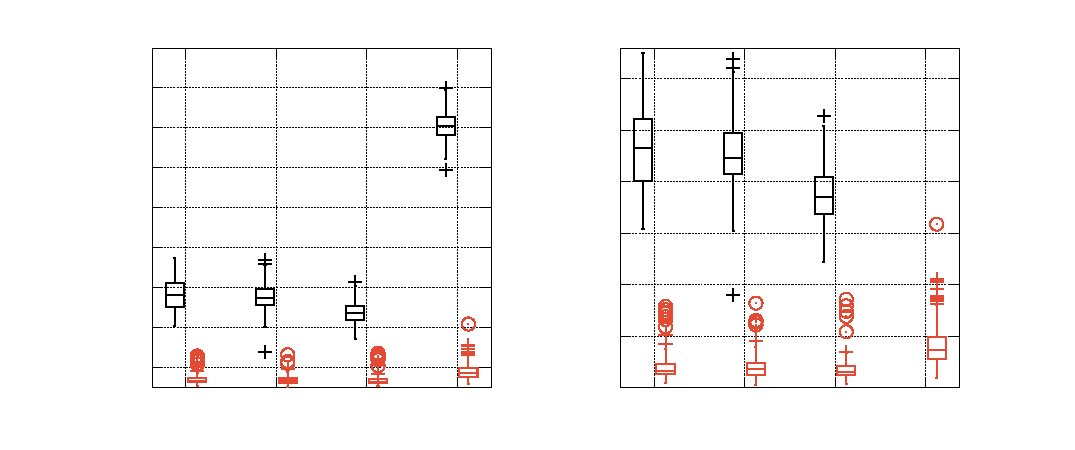
\includegraphics[scale=0.5]{./figures/slides/ch4/experiments/boxplots/warehouse_mean_total_errors_per_selection}}%
    \gplfronttext
  \end{picture}%
\endgroup

  \end{figure}

\note{\scriptsize
Σε αυτή τη διαφάνεια βλεπουμε τις κατανομές των μέσων σφαλμάτων εκτίμησης ανά
  διαδρομή για 100 επαναλήψεις σε κάθε περιβάλλον, ανά μέθοδο διαλογής,
  στα αριστερά σε πλήρη άποψη και στα δεξιά σε εστίαση. Με τη συντομογραφία
  $100\%$ εννοούμε την ονομαστική κατάσταση του φίλτρου, της οποίας το σφάλμα
  είναι κατά μέσο όρο μεγαλύτερο από την κατάσταση που σημαίνουμε με μεγαλύτερο
  από μέσο W, η οποία είναι η κατάσταση όπου επιλέγονται να ψηφίσουν μονο
  εκείνα τα σωματίδια των οποίων το βάρος είναι μεγαλύτερο από το μέσο βάρος
  του πληθυσμού. Με τη σειρά της, το σφάλμα αυτής της κατάστασης είναι
  μεγαλύτερο από εκείνη που σημαίνουμε με $10\%$, η οποία είναι η κατάσταση
  όπου μόνο το $10\%$ των βαρύτερων σωματιδίων ψηφίζουν. Το αντιδιαισθητικό σε
  αυτά τα πειράματα είναι πως η κατάσταση όπου η εκτίμηση διαμορφώνεται από το
  σωματίδιο που εμφανίζει το μεγαλύτερο βάρος, η οποία σημαίνεται με τη λέξη
  τοπ, δηλαδή η εκτίμηση που εξηγεί την τρέχουσα μέτρηση στο μεγαλύτερο βαθμό
  με βάση το μοντέλο παρατήρησης, εμφανίζει το μεγαλύτερο σφάλμα ανάμεσα σε
  όλες τις διαμορφώσεις. Το συμπέρασμα που αντλούμε από αυτά τα αποτελέσματα
  είναι ότι ναι μεν επιβεβαιώνεται η υπόθεσή μας, αλλά η βελτίωση είναι μικρή,
  και έχει ένα οριακό σημείο ως προς τον αριθμό των πιο βαρέων σωματιδίων που
  επιλέγονται.}


\end{frame}
